\chapter{Formatting Text}

\section{Emphasis}

\section{Sizes}

The default text size is controlled by your document class.
It is usually ten points,\punckern\footnote{The standard digital publishing
point, sometimes called the PostScript point, is \otffrac{1}{72} of an inch.
\LaTeX{}, for historical reasons, defines its point (\texttt{pt})
as \otffrac{100}{7227} of an inch
and the former as a ``big point''\quotekern, or \texttt{bp}.}
but this can be adjusted by passing additonal arguments to
\verb|\documentclass|.\punckern\footnote{The standard \LaTeX{} classes accept
\texttt{10pt}, \texttt{11pt}, or \texttt{12pt}.
KOMA Script classes accept arbitrary sizes with
\monobox{fontsize=<size>}.}
To scale text relative to this size, use the following commands:
\begin{leftfigure}
\lm
\renewcommand{\arraystretch}{1.5}
\begin{tabular}{l l}
\verb|\tiny| & \tiny Example Text \\
\verb|\scriptsize| & \scriptsize Example Text \\
\verb|\footnotesize| & \footnotesize Example Text \\
\verb|\small| & \small Example Text \\
\verb|\normalsize| & \normalsize Example Text \\
\verb|\large| & \large Example Text \\
\verb|\Large| & \Large Example Text \\
\verb|\LARGE| & \LARGE Example Text \\
\verb|\huge| & \huge Example Text \\
\verb|\Huge| & \Huge Example Text \\
\end{tabular}
\end{leftfigure}
There is some subtlety here that you may not have noticed.
\LaTeX's default type family, Latin Modern,\punckern\footnote{Latin Modern is
an OpenType rendition of \LaTeX's original type family, Computer Modern.}
comes in multiple \introduce{optical sizes}.
Smaller fonts have thicker strokes, exaggerated features,
and more generous spacing to improve legibility at their size.
\begin{leftfigure}
\fontspec{lmroman5-regular} If you magnify 5 point type
\fontspec{lmroman10-regular} and place the result next to normal 10 point type,
the differences are immediately noticeable.
\end{leftfigure}
Since this requires much more work from the type designer,
many digital typefaces---even professional ones---lack this
feature.\punckern\footnote{If you are fortunate enough \emph{to} have
a typeface with multiple optical sizes, \XeLaTeX{}
and \LuaLaTeX{} can make good use of them! See \chapref{fonts}.}

Points don't tell the whole story, however.
Each font has its own proportions, which can make a huge difference
in its perceived size.
Shown below are some common terms:
\begin{centerfigure}
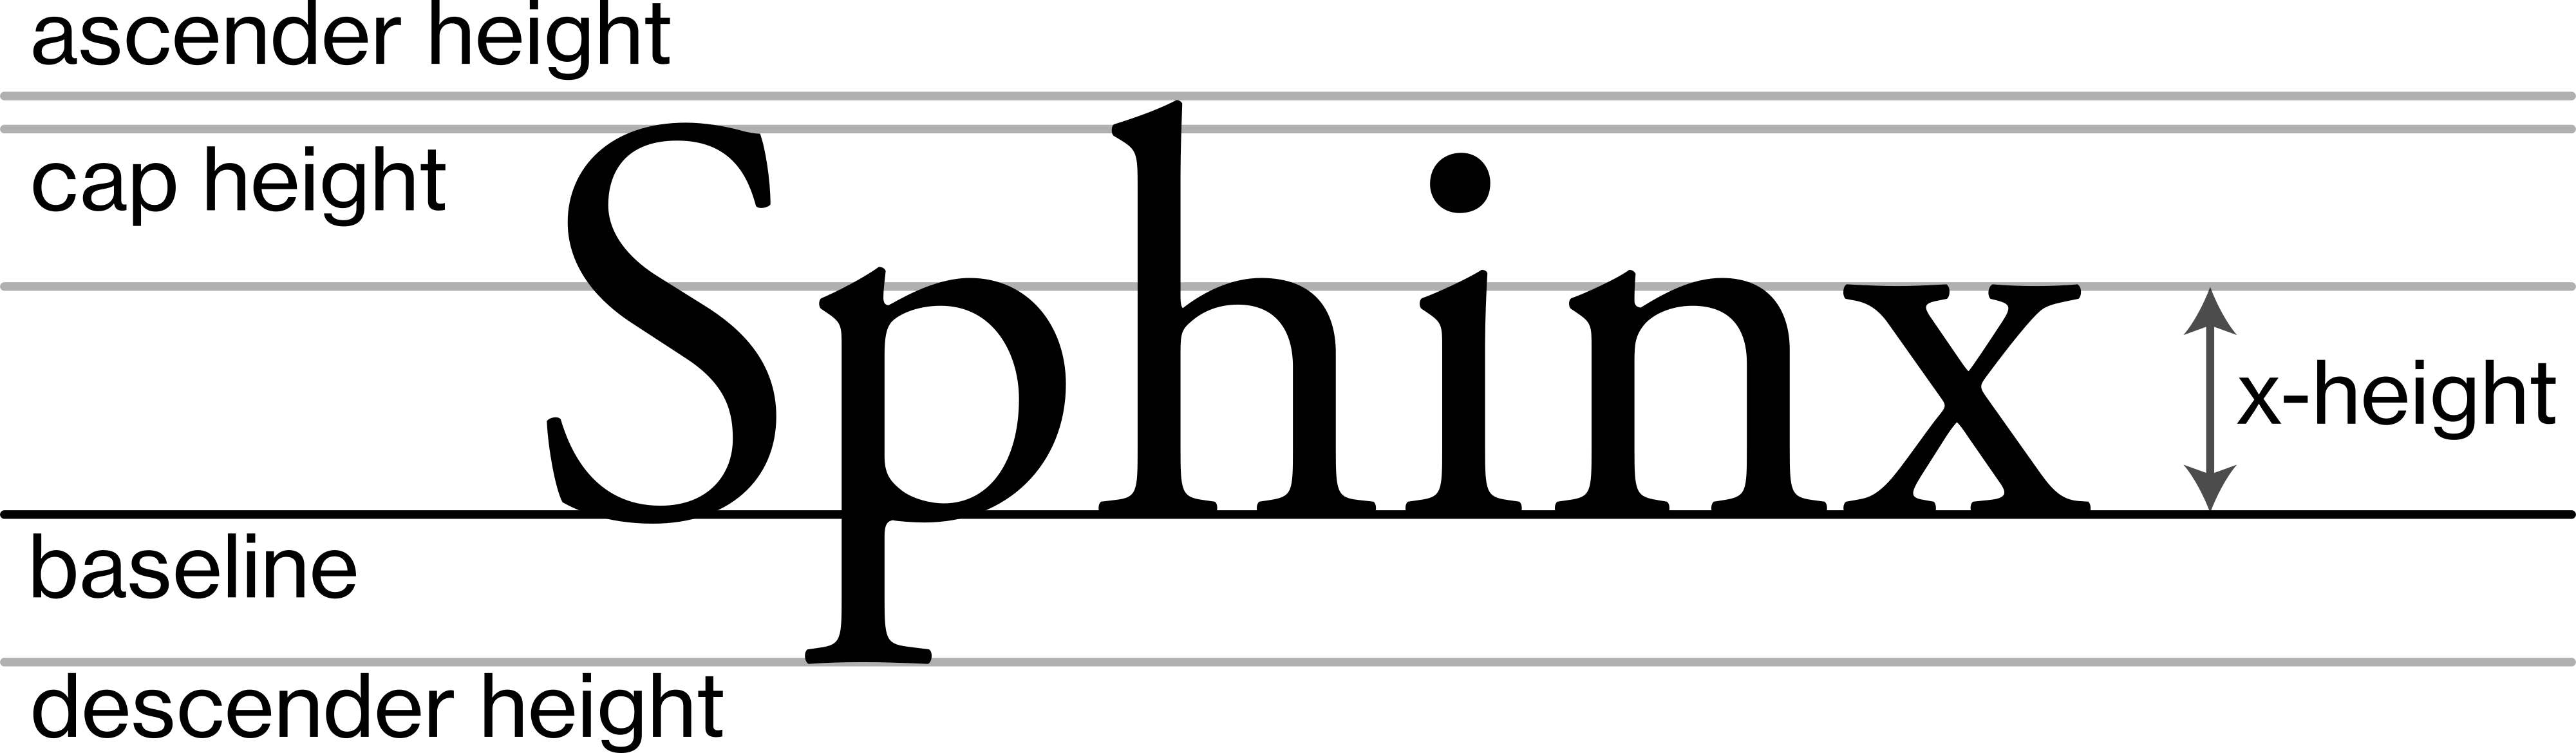
\includegraphics[keepaspectratio,width=0.65\textwidth]{heights.png}

\captionof{figure}{Text sits on the \introduce{baseline},
rises to the \introduce{ascender height},
and drops to the \introduce{descender height}.
The \introduce{cap height} refers to the size of uppercase letters,
and the \introduce{x-height} refers to the size of lowercase letters.}
% For size reference:
%{\sffamily\fontsize{8pt}{8pt}\selectfont This is 8-point text.}
\end{centerfigure}
Different fonts vary wildly in these metrics,
resulting in very different looks at the same point size.
Compare Garamond, {\fontspec{Latin Modern Roman} Latin Modern},
and {\fontspec{NHaasGroteskTXPro-55RG}Helvetica}, all at 10\,pt.
%When multiple {\large sizes} {\footnotesize or} {\sffamily\small fonts}
%are set on the same line, their baselines are aligned.

If the previous commands aren't enough, you can create custom sizes with
\verb|\fontsize|, which takes the desired size and distance between baselines.
\verb|\fontsize| must be followed with \verb|\selectfont| to take effect.
For example, \verb|\fontsize{30pt}{30pt}\selectfont|
gives:
\begin{leftfigure}
\lm
\fontsize{30pt}{30pt}\selectfont
large type with no extra \\
space between lines
\end{leftfigure}
{\fontsize{10pt}{10pt}\selectfont
Note that without extra spacing,
or \introduce{leading},\punckern\footnote{This term comes from the days of
metal type, when strips of lead were inserted
between lines to give them extra spacing.}
descenders from one line nearly collide with ascenders and capitals from
the line below.
Leading is important---without it, blocks of text become uncomfortable to
read, especially at normal body sizes.\par}
Let your type breathe.\punckern\footnote{For a discussion on optimal leading,
see \textit{Practical Typography}, listed in Appendix~\ref{resources}.}
